\documentclass[a4paper,12pt]{memoir}
\usepackage{cmap}
\usepackage[utf8]{inputenc}
\usepackage[russian]{babel}
\usepackage[TS1,T2A]{fontenc}
\usepackage{indentfirst}%делать отступ в начале параграфа
\usepackage{amsmath,amssymb,amsfonts,amscd,amsthm}% расширенный набор матем. символов
\usepackage{bm}
\usepackage{color}% для использования цвета
\usepackage{graphicx} % для вставки рисунков
\usepackage{listingsutf8} % это лучше, чем verbatim
%\usepackage{russmath} % для корректного переноса матем. формул
\usepackage{hyperref}
\usepackage{pgf}

\long\def\title#1#2#3#4#5#6#7{
\mainmatter
\noindent
\thispagestyle{empty}

\vspace*{-\headheight}\vspace*{-\headsep}

\begin{center}
\textsc{
министерство образования и науки российской федерации\\
\textbf{\small{федеральное государственное автономное образовательное\\
учреждение высшего профессионального образования\\
<<Национальный исследовательский ядерный университет «МИФИ»}\\
(НИЯУ МИФИ)}\\
кафедра информационных систем и технологий\\
}

\vspace{4cm plus 1mm minus 1mm}


{\LARGE\textbf{КУРСОВАЯ РАБОТА}}

\vspace{1cm plus 1mm minus 1mm}

{\large
по дисциплине <<#1>>\\
на тему <<#2>>\\

\vfill

\begin{tabular}{l}
Группа\\
\\
Студент\\
\\
Руководитель работы\\
#5\\
\end{tabular}
\hfill
\begin{tabular}{l}
#3\\
\\
#4\\
\\
\\
#6\\
\end{tabular}

\vspace{3cm plus 1mm minus 1mm}

Москва #7
}

\newpage

% Обратная сторона титульного листа
\setcounter{page}{2}

\vspace*{1cm}
\section*{Аннотация}
\begin{quote}
Работа посвящена модификации проектов «Компилятор формул»,
«Интерпретатор арифметических выражений», «Выпуклая оболочка» и
«Изображение проекции полиэдра». В первом из этих проектов решалась
задача расширения языка стекового калькулятора выражений операцией побитового сдвига.
Модификация второго пректа требовала решения задачи расширения итерпретатора
арифметических выражений, расширенного операциями побитового сдвига со специальным
приоретом. В проекте «Выпуклая оболочка» вычислялось расстояние от выпуклой оболочки до стандартного прямоугольника и количество острых углов в выпуклой оболочке. В последнем из проектов
определялась сумма периметров частично видимых граней полиэдра.

\end{quote}

\tableofcontents*

\newpage

\end{center}

}

\def\+{\hskip 0.15mm}

\lccode`\-=`\-\defaulthyphenchar=127 %перенос слов с дефисами

\emergencystretch=2pt
\hfuzz=0.8pt

%Размер страницы
\settrimmedsize{297mm}{210mm}{*} % a4paper: 297mm * 210mm%

% Оформление страницы
\pagestyle{plain}

%Размер текста
\settypeblocksize{46\baselineskip}{160mm}{*}
\setulmargins{*}{*}{1}
\setlrmargins{*}{*}{1}
\checkandfixthelayout
\typeoutlayout

\newcommand{\link}[1]{\texttt{#1}}

% Нумерация рисунков и таблиц сплошная по всему документу
\renewcommand{\thefigure}{\arabic{figure}}
\renewcommand{\theequation}{\arabic{equation}}
\addtodef{\mainmatter}{}{%
\counterwithout{figure}{section}%
\counterwithout{table}{section}%
%\counterwithout{longtable}{section}%
}

% Оформление секций
\makeatletter
\renewcommand*{\thesection}{\@arabic\c@section.}
\setsecnumformat{\csname the#1\endcsname\space}
\makeatother

\renewcommand{\thesubsection}{\large\arabic{subsection}}
%\setsecheadstyle{\centering\scshape}
\setbeforesecskip{\onelineskip}
\setaftersecskip{0.6\onelineskip}

%В подписях к рисункам разделитель - точка
%\captiondelim{ }
\captiondelim{.\space}
%Уменьшенный шрифт для подписей
\captionnamefont{\small\itshape}
\captiontitlefont{\small}
% Пробел до и после рисунка
\setlength{\intextsep}{6mm}
%\setlength{\textfloatsep}{3mm}
%Пробел до и после подписи к рисунку
\setlength{\abovecaptionskip}{2mm}
\setlength{\belowcaptionskip}{0mm}
\changecaptionwidth\captionwidth{0.85\linewidth}

%Убираем большие расстояния по вертикали в списках
\tightlists

% Оформление списка литературы
\setbiblabel{[#1]\hfill}
\renewcommand{\bibsection}{%
  \section*{Список литературы и интернет-ресурсов}
  \prebibhook}

\lstset{language=Ruby,inputencoding=utf8/koi8-r,basicstyle=\small,
stringstyle=\ttfamily,xleftmargin=1cm}

\begin{document}
\renewcommand{\contentsname}{{\Large{Содержание}\hfill}}

\title{Алгоритмы и структуры данных}
{Расширение языков стекового калькулятора и интерпретатора арифметических
выражений операцией побитового сдвига.
Вычисление периметра и площади части выпуклой оболочки, расположенной в
верхней полуплоскости. Нахождение суммы длин полностью видимых рёбер полиэдра}
{K04-361}
{А.\+Ю.~Шедько}
{к.ф.-м.н., доцент}
{Е.\+А.~Роганов}
{2016}

\section{Введение}

В проектах «Компилятор формул» и «Интерпретатор арифметических
выражений» были решены задачи расширения языков стекового калькулятора
и интерпретатора арифметических выражений операциями побитового сдвига.
Применена структура данных <<хэш-таблица>>.Решение задачи требовало представления
о формальных грамматиках, основы ООП и знания языка Ruby.

Проект «Выпуклая оболочка»\cite{convex} решает задачу индуктивного перевычисления выпуклой оболочки последовательно поступающих точек плоскости и таких её характеристик, как периметр и площадь. Целью данной работы является
индуктивное вычисление расстояние до наперёд заданного стандартного прямоугольника
и количества острых улов выпуклой оболочки. Применено два специфических алгоритма,
значительно ускоряющих вычисление расстояние от прямоугольника до
отрезка~\cite{seginters} и проверку пересечения прямоугольника и
отрезка (алгоритм Лианга-Барски)~\cite{barsky}. Решение этой задачи требует знания
теории индуктивных функций, основ аналитической геометрии и векторной алгебры
и языка Ruby~\cite{ruby}.

Проект «Изображение проекции полиэдра»~\cite{polyedr}~--- пример
классической задачи, для успешного решения которой необходимо знакомство с
основами вычислительной геометрии. Задачей, решаемой в данной работе, является
модификация эталонного проекта с целью определения суммы длин полностью видимых
рёбер заданного полиэдра. Для этого необходимы хорошее понимание ряда разделов
аналитической геометрии и векторной алгебры, основ объектно-ориентированного
программирования и языка Ruby.

Для подготовки пояснительной записки необходимо знакомство с программой компьютерной вёрстки \LaTeX~\cite{rlatex}, умение набирать математические формулы~\cite{texbook} и включать в документ графические изображения и исходные
коды программ.

Общее количество строк в рассмотренных проектах составляет около $190$, из которых $28$ были изменены или добавлены автором в процессе работы над задачами модификации.

%\section{Рекомендации по оформлению работы}

Этот раздел содержит рекомендации по оформлению пояснительной записки
и примеры использования различных \LaTeX-конструкций. При подготовке
реального отчёта о выполненной работе данный раздел, естественно, должен
быть опущен.

\subsection*{Общие замечания по структуре курсовой работы}

Обычно в любой работе должно быть \emph{не менее} трёх разделов. Приложение
(или приложения) с текстами программ \emph{не должны} составлять б\'{о}льшую
часть работы. Хорошо, когда в работе имеются таблицы, рисунки или диаграммы,
«снимки экрана» и математические формулы. Возможна, например, такая 
структура работы:

\begin{itemize}
\item введение, содержащее постановку решаемой задачи (или задач);
\item изложение необходимых для решения задачи теоретических аспектов;
\item описание используемых структур данных и применяемых алгоритмов;
\item возможные обобщения рассматриваемой задачи;
\item приложения с фрагментами программ;
\item список литературы и интернет-ресурсов.
\end{itemize}

\subsection*{Рекомендации по использованию \LaTeX}

Для подготовки пояснительной записки следует применять \LaTeX\ и пакет 
\texttt{memoir}. Настоятельно рекомендуется использовать в исходных 
\TeX-файлах кодировку \texttt{UTF-8}. При этом длина большей части строк в 
этих файлах не должна превосходить 79 символов. Рекомендуется 
использовать только те команды переключения шрифтов, которые поддерживаются
пакетом \verb|memoir| без опции \verb|oldfontcommands|. 

При создании pdf-файла используются головной файл \texttt{paper.tex},
в котором подключаются дополнительные 
пакеты, определяются размеры полей, стиль оформления страниц и целый ряд иных 
параметров и макросов, включая макрос, задающий титульный лист пояснительной
записки.

При наборе русского текста перед знаками препинания пробел не ставится, 
а после них~--- ставится всегда. Следует использовать букву «ё», 
кавычки-ёлочки 
(например, \verb|«Информационные технологии и моделирование»|) и
прямой шрифт при наборе единиц измерения (кг, м/сек${}^2$).
При записи инициалов людей рекомендуется применять «сверхтонкий пробел» 
(\verb|\+|) между именем и отчеством и «неразрывный пробел» (\verb|~|) между
отчеством и фамилией: \verb|И.\+И.~Иванов|. 

Следует использовать по назначению тире
(---), «указатель диапазона» (--), дефис (-) и математический знак «минус»
($-$). Перед тире рекомендуется ставить «неразрывный
пробел», а после него~--- обычный: \verb|после него~--- обычный|. Указатель
диапазона применяется, например, при указании страниц: стр. 15--17
(набирается как \verb|стр. 15--17|). Для набора дефиса необходим минус: 
\verb|объектно-ориентированный|, а для получения знака операции  «минус»
требуется применять математический режим: число $-2$ набирается как
\verb|$-2$|. 

Сокращения словосочетаний «и так далее» и «и тому подобное», которые
завершают предложение, набираются так: \verb|и~т.\,д.|, \verb|и~т.\,п.|
Не рекомендуется использовать подобные сокращения для словосочетаний,
находящихся в середине предложения. Для набора нумерованных списков 
целесообразно использовать окружение \verb|\enumerate| в~следующем виде:
\verb|\begin{enumerate}[1)]|.
Стандартный стиль оформления рисунков и таблиц~--- использование окружений
\verb|figure| и \verb|table|. При этом обязательно следует применять макрос
\verb|caption| для набора подписи. 

При наборе математических формул следует нумеровать только те из них, на
которые имеются ссылки. Для получения полужирного шрифта в математических
формулах можно применять команду \verb|\bm|: $\pi \ne \bm\pi$.

О наборе математики мы уже говорили весьма подробно, поэтому сейчас 
ограничимся лишь двумя примерами. Следующий код
\begin{small}
\begin{verbatim}
$$\int\limits_a^b\frac12 (1+x)^{-3/2}dx=
\left.-\frac{1}{\sqrt{1+x}}\right|_a^b$$
\end{verbatim}
\end{small}
\noindent позволяет получить формулу

$$\int\limits_a^b\frac12 (1+x)^{-3/2}dx=
\left.-\frac{1}{\sqrt{1+x}}\right|_a^b$$

Приведённый ниже фрагмент кода из книги~\cite{roganov-jurists}
является более сложным.
\begin{small}
\begin{verbatim}
Рассмотрим сначала одну из самых простых функций~$y=x^{2}$. Обычно правую
часть в аналитической записи функции обозначают через $f(x)$. Итак, у нас
$f(x)=x^{2}$. Заметим, что значение этой функции в точке $x_{0} = 2$ равно
$y_{0} = 4$, и возьмём на оси $X$ бесконечную последовательность точек с
координатами $x_{n}=2-1/2^{n - 1}$: $x_{1}=2-1=1$; $x_{2}=2-1/2=3/2$;
$x_{3}=2-1/4=1 3/4$; $\ldots$

\noindent
Эта последовательность, как мы выяснили в \S1, имеет предел, равный двум:
$\displaystyle\lim_{n \to \infty } x_n = 2$. Найдём значения функции
$f(x)$ в выбранных точках: 
$$\displaylines{
y_1=f(x_1)=f(1)=1;\cr
y_2=f(x_2)=f\left(\dfrac32\right)= \dfrac94;\cr
y_3=f(x_3)=f\left(\dfrac74\right)=\dfrac{49}{16};\cr
\ldots\ldots\ldots\ldots\ldots\ldots\ldots\ldots\ldots;\cr
y_n=f(x_n)=f\left(2-\dfrac{1}{2^{n-1}}\right)=
\left(2-\dfrac{1}{2^{n-1}}\right)^2=4-\dfrac{1}{2^{n-3}}+\dfrac{1}{2^{2n-2}}.
}$$
\end{verbatim}
\end{small}
\noindent Вот во что он превращается:

Рассмотрим сначала одну из самых простых функций~$y=x^{2}$. Обычно правую
часть в аналитической записи функции обозначают через $f(x)$. Итак, у нас
$f(x)=x^{2}$. Заметим, что значение этой функции в точке $x_{0} = 2$ равно
$y_{0} = 4$, и возьмём на оси $X$ бесконечную последовательность точек с
координатами $x_{n}=2-1/2^{n - 1}$: $x_{1}=2-1=1$; $x_{2}=2-1/2=3/2$;
$x_{3}=2-1/4=1 3/4$; $\ldots$

\noindent
Эта последовательность, как мы выяснили в \S1, имеет предел, равный двум:
$\displaystyle\lim_{n \to \infty } x_n = 2$. Найдём значения функции
$f(x)$ в выбранных точках: 
$$\displaylines{
y_1=f(x_1)=f(1)=1;\cr
y_2=f(x_2)=f\left(\dfrac32\right)= \dfrac94;\cr
y_3=f(x_3)=f\left(\dfrac74\right)=\dfrac{49}{16};\cr
\ldots\ldots\ldots\ldots\ldots\ldots\ldots\ldots\ldots;\cr
y_n=f(x_n)=f\left(2-\dfrac{1}{2^{n-1}}\right)=
\left(2-\dfrac{1}{2^{n-1}}\right)^2=4-\dfrac{1}{2^{n-3}}+\dfrac{1}{2^{2n-2}}.
}$$

Теперь рассмотрим пример простой таблицы, которая строится с помощью окружения
\verb|tabular|, и состоит из трёх столбцов. Содержимое каждого столбца может
центрироваться (\verb|c|), либо прижиматься к левому (\verb|l|) или правому
(\verb|r|) краям. Символ~\verb|&| указывает на границу между столбцами, а
символы \verb|\\| --- на конец строки таблицы. Следует понимать, что в таблице 
вовсе не обязаны присутствовать горизонтальные и вертикальные линии. Вот как
можно задать грамматику, используя именно такую таблицу:

\medskip
\noindent\hspace{2cm}
\begin{tabular}{rll}
$\alpha \rightarrow$ & $ab\beta$\\
$\beta  \rightarrow$ & $\alpha\mid\gamma$\\
$\gamma \rightarrow$ & $\beta\mid\varepsilon$\\
\end{tabular}
\medskip

\noindent Исходный код для получения этой таблицы имеет следующий вид:

\begin{small}
\begin{verbatim}
\noindent\hspace{2cm}
\begin{tabular}{rll}
$\alpha \rightarrow$ & $ab\beta$\\
$\beta  \rightarrow$ & $\alpha\mid\gamma$\\
$\gamma \rightarrow$ & $\beta\mid\varepsilon$\\
\end{tabular}
\end{verbatim}
\end{small}

Более сложной является таблица~\ref{tabl:crayfish}, позаимствованная из книги
С.\+М.~Львовского~\cite{rlatex}. Заметим, что эта таблица снабжена
подписью (caption) и меткой (label), позволяющей ссылаться на неё.

\begin{table}[ht!]
\caption{Известная шутка М.\+М.~Жванецкого}\label{tabl:crayfish}
\begin{center}
\begin{tabular}{|p{5cm}|p{5cm}|}
\hline
\multicolumn{2}{|c|}{\large\textbf{Я видел раков}}\\
\hline
Вчера: & Сегодня: \\
\hline
Маленькие, но по три рубля, но очень
маленькие, но по три, но очень маленькие.
&
Большие, но по пять рублей, но большие, но
по пять рублей, но очень большие,
но по пять.\\
\hline
\end{tabular}
\end{center}
\end{table}

\noindent 
Вот каков исходный код таблицы~\ref{tabl:crayfish}:

\begin{small}
\begin{verbatim}
\begin{table}[ht!]
\caption{Известная шутка М.\+М.~Жванецкого}\label{tabl:crayfish}
\begin{center}
\begin{tabular}{|p{5cm}|p{5cm}|}
\hline
\multicolumn{2}{|c|}{\large\textbf{Я видел раков}}\\
\hline
Вчера: & Сегодня: \\
\hline
Маленькие, но по три рубля, но очень
маленькие, но по три, но очень маленькие.
&
Большие, но по пять рублей, но большие, но
по пять рублей, но очень большие,
но по пять.\\
\hline
\end{tabular}
\end{center}
\end{table}
\end{verbatim}
\end{small}

Наиболее правильным вариантом включение изображения (формата \verb|png| или
\verb|jpg|)
в документ является использование окружения \verb|figure|, что
даёт возможность использовать подписи и нумеровать рисунки.

\begin{figure}[ht!]
\begin{center}

\includegraphics[scale=0.6]{images/mephi_logo}
\end{center}
\vspace*{-8mm}
\caption{Логотип МИФИ}\label{fig:mephi_logo}
\end{figure}

\newpage

Исходный код, использованный для включения логотипа МИФИ,
изображённого на рис.~\ref{fig:mephi_logo}, таков:

\begin{small}
\begin{verbatim}
\begin{figure}[ht!]
\begin{center}

\includegraphics[scale=0.6]{images/mephi_logo}
\end{center}
\vspace*{-8mm}
\caption{Логотип МИФИ}\label{fig:mephi_logo}
\end{figure}
\end{verbatim}
\end{small}

Часто бывает полезно включать в документ «снимки экрана», масштабируя
картинку нужным образом. Примером является рис.~\ref{fig:rating}.

\begin{figure}[ht!]
\begin{center}
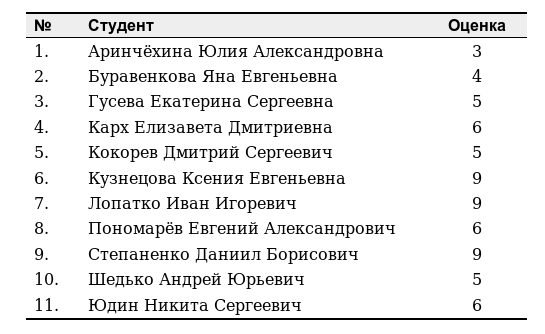
\includegraphics[width=0.6\hsize]{images/rating}
\end{center}
\caption{Оценки за самостоятельную работу}\label{fig:rating}
\end{figure}

Иногда можно воспользоваться возможностями самого \LaTeX'а,
позволяющего создавать «псевдорисунки». Вот исходный код
рис.~\ref{fig:simple}:

\begin{small}
\begin{verbatim}
\begin{picture}(120,80)
% Границы изображения:
\put(0,0){\line(1,0){120}}
\put(0,80){\line(1,0){120}}
\put(0,0){\line(0,1){80}}
\put(120,0){\line(0,1){80}}
%
% Оси координат:
\put(40,25){\begin{picture}(40,40)%
              \put(20,0){\vector(0,1){40}}
              \put(0,20){\vector(1,0){40}}
              \put(40,22){$x$}
              \put(22,40){$y$}
            \end{picture}}
\end{picture}
\end{verbatim}
\end{small}

\begin{figure}[ht!]
\begin{center}
\begin{picture}(120,80)
% Границы изображения:
\put(0,0){\line(1,0){120}}
\put(0,80){\line(1,0){120}}
\put(0,0){\line(0,1){80}}
\put(120,0){\line(0,1){80}}
%
% Оси координат:
\put(40,25){\begin{picture}(40,40)%
              \put(20,0){\vector(0,1){40}}
              \put(0,20){\vector(1,0){40}}
              \put(40,22){$x$}
              \put(22,40){$y$}
            \end{picture}}
\end{picture}
\end{center}
\caption{Простой псевдорисунок}\label{fig:simple}
\end{figure}

Гораздо более интересным является рис~\ref{fig:cos_acos}, 
исходный код для которого создан с помощью небольшого скрипта,
написанного на языке Ruby и приведённого в приложении.

\begin{figure}[ht!]
\begin{center}
% Цвет для клеточек
\definecolor{gridcolor}{cmyk}{0.30,0.00,0.0,0.0}
% Основной цвет гистограмм и графиков
\definecolor{plot1}{cmyk}{0.9,0.5,0.0,0.0} 
% Второй цвет гистограмм и графиков
\definecolor{plot2}{cmyk}{0.0,0.60,0.70,0.0} 
% Толщина линии у клеточек
\newlength\gridwidth
\setlength{\gridwidth}{0.8pt}
% Макрос для включения клеточек
\newcommand{\mygrid}[4]{
\begin{pgfscope}
\pgfsetlinewidth{\gridwidth}\color{gridcolor}
\pgfgrid[stepx=0.5cm,stepy=0.5cm]{\pgfxy(#1,#2)}{\pgfxy(#3,#4)}
\end{pgfscope}
}
% Толщина линии у графиков
\newlength\plotwidth
\setlength{\plotwidth}{1.2pt}

% Собственно картинка
\begin{pgfpicture}{0mm}{0mm}{ 69.333mm}{ 69.333mm}
\pgfsetxvec{\pgfpoint{  8.000mm}{0mm}}
\pgfsetyvec{\pgfpoint{0mm}{  8.000mm}}
\begin{pgftranslate}{\pgfpoint{ 34.667mm}{ 34.667mm}}
%
\mygrid{-4.2}{-4.2}{4.2}{4.2}
%
\pgfsetendarrow{\pgfarrowsingle}
\pgfxyline( -4.333,0)(  4.333,0)
\pgfxyline(0, -4.333)(0,  4.333)
\pgfclearendarrow
%
\pgfputat{\pgfxy( 0.400, -0.480)}{\pgfbox[right,base]{\small$O$}}
\pgfputat{\pgfxy(  4.333, -0.480)}{\pgfbox[right,base]{\small $X$}}
\pgfputat{\pgfxy( -0.100,  4.333)}{\pgfbox[right,top]{\small $Y$}}
%
\pgfxyline(1, -0.100)(1,  0.100)
\pgfputat{\pgfxy(  1, -0.480)}{\pgfbox[center,base]{\small $1$}}
\pgfxyline(-1, -0.100)(-1,  0.100)
\pgfputat{\pgfxy(  -1.000, -0.480)}{\pgfbox[center,base]{\small $-1$}}
\pgfxyline(3.1416, -0.100)(3.1416,  0.100)
\pgfputat{\pgfxy(  3.1416, 0.280)}{\pgfbox[center,base]{\small $\pi$}}
\pgfxyline( -0.100,3.1416)(  0.100,3.1416)
\pgfputat{\pgfxy( 0.400,  3.1416)}{\pgfbox[right,center]{\small $\pi$}}
%
\pgfsetdash{{0.1cm}{0.1cm}}{0cm}
\pgfxyline(3.1416, 0)(3.1416, -1.0)
\pgfxyline(-1,3.1416)(0,3.1416)
\pgfsetdash{}{0cm}
%
\pgfsetdash{{0.2cm}{0.1cm}}{0cm}
\pgfxyline(-1,-1)(3,3)
\pgfsetdash{}{0cm}
%
\color{plot1}
\pgfxycurve( -4.333, -0.370)( -4.222, -0.473)( -4.111, -0.570)( -4.000, -0.654)
\pgfxycurve( -4.000, -0.654)( -3.889, -0.738)( -3.778, -0.810)( -3.667, -0.865)
\pgfxycurve( -3.667, -0.865)( -3.556, -0.921)( -3.444, -0.960)( -3.333, -0.982)
\pgfxycurve( -3.333, -0.982)( -3.222, -1.003)( -3.111, -1.006)( -3.000, -0.990)
\pgfxycurve( -3.000, -0.990)( -2.889, -0.974)( -2.778, -0.940)( -2.667, -0.889)
\pgfxycurve( -2.667, -0.889)( -2.556, -0.839)( -2.444, -0.771)( -2.333, -0.691)
\pgfxycurve( -2.333, -0.691)( -2.222, -0.610)( -2.111, -0.517)( -2.000, -0.416)
\pgfxycurve( -2.000, -0.416)( -1.889, -0.315)( -1.778, -0.206)( -1.667, -0.096)
\pgfxycurve( -1.667, -0.096)( -1.556,  0.015)( -1.444,  0.127)( -1.333,  0.235)
\pgfxycurve( -1.333,  0.235)( -1.222,  0.343)( -1.111,  0.447)( -1.000,  0.540)
\pgfxycurve( -1.000,  0.540)( -0.889,  0.634)( -0.778,  0.717)( -0.667,  0.786)
\pgfxycurve( -0.667,  0.786)( -0.556,  0.855)( -0.444,  0.909)( -0.333,  0.945)
\pgfxycurve( -0.333,  0.945)( -0.222,  0.981)( -0.111,  1.000)( -0.000,  1.000)
\pgfxycurve( -0.000,  1.000)(  0.111,  1.000)(  0.222,  0.981)(  0.333,  0.945)
\pgfxycurve(  0.333,  0.945)(  0.444,  0.909)(  0.556,  0.855)(  0.667,  0.786)
\pgfxycurve(  0.667,  0.786)(  0.778,  0.717)(  0.889,  0.634)(  1.000,  0.540)
\pgfxycurve(  1.000,  0.540)(  1.111,  0.447)(  1.222,  0.343)(  1.333,  0.235)
\pgfxycurve(  1.333,  0.235)(  1.444,  0.127)(  1.556,  0.015)(  1.667, -0.096)
\pgfxycurve(  1.667, -0.096)(  1.778, -0.206)(  1.889, -0.315)(  2.000, -0.416)
\pgfxycurve(  2.000, -0.416)(  2.111, -0.517)(  2.222, -0.610)(  2.333, -0.691)
\pgfxycurve(  2.333, -0.691)(  2.444, -0.771)(  2.555, -0.838)(  2.667, -0.889)
\pgfxycurve(  2.667, -0.889)(  2.778, -0.940)(  2.889, -0.974)(  3.000, -0.990)
\pgfxycurve(  3.000, -0.990)(  3.111, -1.006)(  3.222, -1.003)(  3.333, -0.982)
\pgfxycurve(  3.333, -0.982)(  3.444, -0.961)(  3.555, -0.921)(  3.667, -0.865)
\pgfxycurve(  3.667, -0.865)(  3.778, -0.810)(  3.889, -0.738)(  4.000, -0.654)
\pgfxycurve(  4.000, -0.654)(  4.111, -0.570)(  4.222, -0.473)(  4.333, -0.370)
%
\pgfsetlinewidth{\plotwidth}
\pgfxycurve(  0.000,  1.000)(  0.131,  1.000)(  0.263,  0.974)(  0.394,  0.923)
\pgfxycurve(  0.394,  0.923)(  0.526,  0.873)(  0.657,  0.798)(  0.788,  0.705)
\pgfxycurve(  0.788,  0.705)(  0.920,  0.612)(  1.051,  0.500)(  1.183,  0.379)
\pgfxycurve(  1.183,  0.379)(  1.314,  0.257)(  1.445,  0.125)(  1.577, -0.006)
\pgfxycurve(  1.577, -0.006)(  1.708, -0.137)(  1.840, -0.269)(  1.971, -0.390)
\pgfxycurve(  1.971, -0.390)(  2.102, -0.511)(  2.234, -0.621)(  2.365, -0.713)
\pgfxycurve(  2.365, -0.713)(  2.497, -0.806)(  2.628, -0.879)(  2.759, -0.928)
\pgfxycurve(  2.759, -0.928)(  2.891, -0.977)(  3.022, -1.002)(  3.154, -1.000)
%
\color{plot2}
\pgfxycurve(  1.000,  0.000)(  1.000,  0.131)(  0.974,  0.263)(  0.923,  0.394)
\pgfxycurve(  0.923,  0.394)(  0.873,  0.526)(  0.798,  0.657)(  0.705,  0.788)
\pgfxycurve(  0.705,  0.788)(  0.612,  0.920)(  0.500,  1.051)(  0.379,  1.183)
\pgfxycurve(  0.379,  1.183)(  0.257,  1.314)(  0.125,  1.445)( -0.006,  1.577)
\pgfxycurve( -0.006,  1.577)( -0.137,  1.708)( -0.269,  1.840)( -0.390,  1.971)
\pgfxycurve( -0.390,  1.971)( -0.511,  2.102)( -0.621,  2.234)( -0.713,  2.365)
\pgfxycurve( -0.713,  2.365)( -0.806,  2.497)( -0.879,  2.628)( -0.928,  2.759)
\pgfxycurve( -0.928,  2.759)( -0.977,  2.891)( -1.002,  3.022)( -1.000,  3.154)
\end{pgftranslate}
\end{pgfpicture}

\end{center}
\caption{Графики функций $y=\cos x$ и $y=\arccos x$}\label{fig:cos_acos}
\end{figure}

Один из простейших способов включения в документ листинга программы~--- 
использование окружения \verb|verbatim|. При этом полезно немного
уменьшить размер используемого шрифта:

\begin{small}
\begin{verbatim}
y1 = 0
begin
  print "x -> "
  y1,y2 = 1,readline.to_i
  while true
    print "x -> "
    x = readline.to_i
    if x == y2
      y1 += 1
    elsif x > y2
      y1,y2 = 1,x
    end
  end
rescue EOFError
  puts "\nКол-во макс. = #{y1}"
end
\end{verbatim}
\end{small}

Часто исходные тексты программ содержат символы табуляции, которые
правильно интерпретируются текстовыми редакторами, но «приводят в
замешательство» \TeX. Для того чтобы получить правильно отформатированный
листинг программы, следует предварительно заменить в ней все символы табуляции
на пробелы либо вручную, либо с помощью утилиты \verb|expand|.

Более правильным способом включения текста программы является использование
окружения \verb|verbatiminput|. При этом
включаемый текст должен быть размещён в отдельном файле, имя которого и
указывается в качестве параметра окружения. Вот пример:

\begin{small}
\begin{verbatim}
\begin{small}
\verbatiminput{programms/binsearch.rb}
\end{small}
\end{verbatim}
\end{small}

Результат выполнения этих команд имеет следующий вид:

\begin{small}
\verbatiminput{programms/binsearch.rb}
\end{small}


\section{Модификация проекта «Компилятор формул»}
\subsection{Постановка задачи}
В предположении, что язык стекового калькулятора
расширен операциями L (left) и R (right),
реализующими побитовый сдвиг влево и вправо соответственно, компилировать
формулы, содержащие операции \verb|<<| и \verb|>>|.

\subsection{Теоретические аспекты}
С формальной точки зрения компилятор представляет собой программную реализацию
некоторой функции $\tau\colon L_1 \rightarrow L_2$, действующей из множества
цепочек одного языка $L_1$ в множество цепочек другого $L_2$ таким образом, что
$\forall \omega \in L_1$ {\em семантика цепочек $\omega$ и $\tau(\omega)\in L_2$
 совпадает.}

Для решения задачи необходимо задать грамматики, описывающие языки стекового
калькулятора и компилятора, соответственно $G_0$ и $G_s$:

$G_0$:
\medskip
\noindent\hspace{2cm}
\begin{tabular}{rcccccll}
\verb|S| $\rightarrow$ & \verb|F| &$\mid$& \verb|SRF|&$\mid$&\verb|SLF|\\
\verb|F| $\rightarrow$ & \verb|T| &$\mid$& \verb|F+T|&$\mid$&\verb|F-T|\\
\verb|T| $\rightarrow$ & \verb|M| &$\mid$& \verb|T*M|&$\mid$&\verb|T/M|\\
\verb|M| $\rightarrow$ & \verb|(S)|&$\mid$& \verb|V|\\
\verb|V| $\rightarrow$ & a &$\mid$& b &$\mid$& \dots &$\mid$& z\\
\end{tabular}
\medskip

$G_s$:
\medskip
\noindent\hspace{2cm}
\begin{tabular}{rll}
\verb|e| $\rightarrow$ & \verb|ee+| $\mid$ \verb|ee-|$\mid$ \verb|ee*| $\mid$ \verb|ee/| $\mid$ \verb|ee>>|$\mid$ \verb|ee<<|$\mid$\\
&$\mid$ a $\mid$ b $\mid \dots \mid$ z
\end{tabular}

\noindent{где $L$, $R$ соответствуют \verb|<<|, \verb|>>|, т.\,е. сдвигу влево и вправо,
а $S$ --- классу сдвигаемых выражений (ассоциативность аналогична \verb|+| и \verb|-|)}.

Нужный нам компилятор $\tau$ представляет собой программную реализацию отображения из
множества цепочек языка $L(G_0)$ в множество цепочек языка $L(G_s)$ По этой причине его можно
рассматривать, как функцию на пространстве последовательностей. Легко понять,
что эта функция не индуктивна.

Построим индуктивное расширение функции, чтобы с его помощью реализовать однопроходный алгоритм, осуществляющий нужный нам перевод. Заметим, что любую
правильную формулу можно откомпилировать с соблюдением следующих двух условий:
\begin{itemize}
\item переменные в выходной цепочке (программе для стекового калькулятора) будут идти
в том же порядке, что и переменные в исходной формуле;
\item все операции в выходной цепочке будут расположены позже соответствующих им
операций в исходной формуле.
\end{itemize}

Любую формулу можно компилировать так: встретив имя переменной, немедленно
записывать его в массив, где мы будем накапливать результат компиляции, а
встретив знак операции или скобку, записывать в этот массив те из предыдущих,
но ещё не обработанных операций (будем называть их \emph{отложенными}), которые
выполнимы в данный момент, после чего «откладывать» и новый знак.

В качестве контейнера для хранения отложенных операций можно использовать стек.
Этот стек и будет содержать ту дополнительную информацию, которая необходима для
индуктивного перевычисления функции $T$ осуществляющей компиляцию исходной формулы.
Основная проблема — понять, что надо делать, когда в исходной формуле встречается
очередная операция или скобка.

Таким образом, встретив в исходной формуле очередной знак операции или скобку,
нужно иногда просто положить её в стек отложенных операций, а иногда — извлечь
предварительно одну или несколько ранее отложенных операций и добавить их в
массив результата. С точки зрения теории индуктивных функций необходимо построить
индуктивное расширение функции $T$ осуществляющей компиляцию исходной формулы, и
найти для неё отображение $G$ обеспечивающее её перевычисление при удлинении входной формулы.

Для построения индуктивной функции компиляции цепочки $\omega$ необходимо разделить
символы на категории: \verb|SYM_LEFT, SYM_RIGHT, SYM_OPER и SYM_OTHER| соответственно.
правила построения таковы:
\begin{itemize}
  \item открывающую скобку всегда помещать в стек, имя переменной --- всегда
  сразу добавлять в массив результата компиляции;
  \item когда в формуле встречается закрывающая скобка нужно все операции,
  появившиеся в ней \emph{после соответствующей ей открывающей скобки}, извлечь
  из стека отложенных операций и добавить в массив результата
  (не забыть также извлечь открывающую скобку);
  \item операции и скобки помещаются в стек в соответствии с приоритетом
  соответствующей операции или скобке. Открывающие скобки имеют наименьший приоритет,
  закрывающие~--- наибольший; для операций он будет описан в дальнейшем.
\end{itemize}
Более подробно см. \cite{compf}

\subsection{Применяемые структуры данных}
Стек, используемый в эталонном проекте, не требует пояснений.
Помимо стека используется константная хэш-таблица (в качестве отображения
между множествами операций двух грамматик). Подробно с работой хеш-таблицы в языке
Ruby можно ознакомиться в документации к языку~\cite{rubydoc} и на соответствующей
странице Википедии.

\subsection{Детали реализации}

Отображение между множествами операций языков калькулятора и компилятора описывается
данной таблицей.
\begin{lstlisting}
CONV_TABLE = {">>" => "R",
              "<<" => "L",
               "+" => "+",
               "-" => "-",
               "/" => "/",
               "*" => "*"}
\end{lstlisting}

Приоритет операций задаётся следующим образом:
\begin{lstlisting}
def priority(c)
  (c == '+' or c == '-') ? 1 : ( c=='L' or c=='R' )? 0 : 2
end
\end{lstlisting}

Этот фрагмент кода устанавливает наименьший приоритет для сдвигов~($0$) и наивысший для
деления и умножения~($2$).

Наиболее значительным является изменение, касающееся обработки символов операций,
а именно обработка символов \verb|>>| и \verb|<<|, так как они занимают два
строковых символа, являясь одним логическим символом. Идея проста: хранить первый
cимвол в обрабатываемой последовательности, соответствующий одной из операций, в
специальной переменной \verb|@op|, а при поступлении следующего символа, если
последовательность составлена верно и этот символ совпадает с
\verb|<| или \verb|>|, записывать его в \verb|@op|. После этого, вне зависимости
от содержимого \verb|@op|, происходит стандартная процедура обработки отложенных
операций с использованием значения \verb|CONV_TABLE[@op]|, которое затем
помещается в стек. После успешной обработки символа \verb|@op| очищается.

\newpage

Код, реализующий обработку символов операций:
\begin{lstlisting}
def process_symbol(c)
  ...
  when SYM_OPER
    if ((c=='>'||c=='<')&&@op=="")
      @op=c
    else
      @op+=c
      process_suspended_operators(CONV_TABLE[@op])
      push(CONV_TABLE[@op])
      @op=""
  end
  ...
end
\end{lstlisting}

Таким образом в язык стекового компилятора добавлена операция побитового сдвига.
\subsection{Возможные обобщения}
Имеет смысл ввести в язык стекового компилятора также остальные побитовые
операции~(\verb|&|, \texttt{\&}, \texttt{|} \verb|^,~|), их логические
аналоги~(\verb|&&|,\texttt{||}).

\section{Модификация проекта «Интерпретатор арифметических выражений»}

\subsection{Постановка задачи}
Вычисляются значения выражений, содержащих битовые операции  \verb|<<| и \verb|>>|,
приоритет первой из которых является минимальным, а второй — максимальным.

\subsection{Теоретические аспекты}
Если компилятор осуществляет перевод с одного языка на другой, то интерпретатор
\emph{вычисляет} значение арифметической формулы, в которой вместо имён переменных
содержатся записанные тем или иным способом числа.

Грамматика $G_0$ из предыдущего пункта должна быть изменена для учёта максимального приоритета операции сдвига вправо:

$G_0$:
\medskip
\noindent\hspace{2cm}
\begin{tabular}{rcccccll}
\verb|S_0| $\rightarrow$ & \verb|F| &$\mid$&\verb|S_0LF|\\
\verb|F| $\rightarrow$ & \verb|T| &$\mid$&\verb|F+T|&$\mid$&\verb|F-T|\\
\verb|T| $\rightarrow$ & \verb|M| &$\mid$&\verb|T*M|&$\mid$&\verb|T/M|\\
\verb|S_1| $\rightarrow$ & \verb|M| &$\mid$& \verb|S_1RF|\\
\verb|M| $\rightarrow$ & \verb|(S_0)|&$\mid$&\verb|V|\\
\verb|V| $\rightarrow$ & a &$\mid$& b &$\mid$& \dots &$\mid$& z\\
\end{tabular}
\medskip

\noindent{\verb|S_0|~--- класс сдвигаемых влево выражений;\newline
\verb|S_1|~--- класс сдвигаемых вправо выражений.}

$G_s$ можно оставить без изменений.

Класс \verb|Calc|, реализующий алгоритм интерпретации арифметических выражений 
может быть построен при помощи уже реализованного класса \verb|Compf|.

Интерпретатор выражений отличается от компилятора тем, что
вместо идентификаторов переменных во входной формуле стоят \emph{числа} и
получаемую выходную формулу необходимо \emph{выполнять} (вместо её печати).
Для того чтобы реализовать стековый калькулятор, естественно, необходим стек.

При появлении на входе цифры, будем помещать её в стек калькулятора \verb|@s|,
а при появлении операции доставать из стека её аргументы и помещать туда результат
её выполнения. На конечном этапе на вершине стека будет находиться результат
выполнения арифметического выражения.

\subsection{Детали реализации}

Здесь также как и в первом проекте применена хеш-таблица для отображения множества
операций стекового компилятора в множество операций языка Ruby.
\begin{lstlisting}
CONV_TABLE = {"R" => ">>",
              "L" => "<<",
              "+" => "+",
              "-" => "-",
              "/" => "/",
              "*" => "*"}
\end{lstlisting}
В соответствии с задачей, приоритет операций был изменён следующим образом:
\begin{lstlisting}
  def priority(c)
    (c == '+' or c == '-') ? 1 : c=='L' ? 0 : (c=='R') ? 3 : 2
  end
\end{lstlisting}
\begin{table}[ht!]
\caption{Приоритет операций}
\begin{center}
\begin{tabular}{|c|c|}
\hline
Операция & Приоритет \\
\hline
\verb|L| & $0$ \\
\hline
\verb|+, -| & $1$ \\
\hline
\verb|*, /| & $2$ \\
\hline
\verb|R| & $3$ \\
\hline
\end{tabular}
\end{center}
\end{table}


\section{Модификация проекта «Выпуклая оболочка»}

\subsection{Постановка задачи}
Требуется модифицировать эталонный проект:
\begin{enumerate}
\item для индуктивного вычисления количества всех острых внутренних углов выпуклой
оболочки~(задача 40).
\item для индуктивного вычисления расстояния от выпуклой оболочки до заданного
стандартного прямоугольника~(Задача 52).
\end{enumerate}
\subsection{Теоретические аспекты}

Задача построения выпуклой оболочки множества точек может быть сформулирована следующим
образом: для множества точек $M$ необходимо найти наименьшее \emph{выпуклое} множество,
включающее $M$. \emph{Выпуклым} будем называть любое множество $M$, удовлетворяющее условию:
$ \forall x_1, x_2 \in M\ [x_1,x_2]\in M.$

\begin{figure}[ht!]
\begin{center}
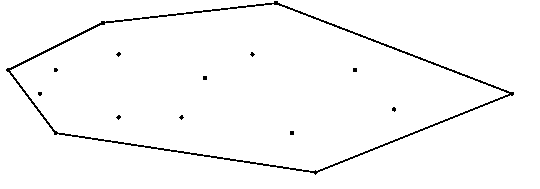
\includegraphics[scale=0.6]{images/conv_a_1}
\end{center}
\vspace*{-8mm}
\caption{Выпуклая оболочка множества точек}\label{fig:convex_hull}
\end{figure}

Пусть $X$~---множество точек на плоскости $\mathbb{R}^2$, $\mathcal{P}$~---
множество всех выпуклых фигур на плоскости. Тогда тройка $(f,g,h)$, где
$f\colon X^* \rightarrow \mathcal{P}$~---
\emph{выпуклая оболочка последовательности точек},
$g\colon X^* \rightarrow \mathbb{N}$~--- \emph{количество острых углов в ней},
$h\colon X^* \rightarrow \mathbb{R}$~---
\emph{расстояние от неё до стандартного прямоугольника}, задаёт индуктивную
функцию $$F\colon X^* \rightarrow \mathcal{P} \times \mathbb{N} \times
\mathbb{R}, F = \begin{pmatrix}f\\ g\\ h\end{pmatrix}.$$
Функция индуктивного перевычисления $G$ представляет собой реализацию следующей
идеи: пусть для некоторой последовательности точек $X^*$ значения $f,g,h$ уже известны.
Тогда при поступлении новой точки $x$ возможны два случая:
либо точка лежит внутри выпуклой оболочки, либо снаружи неё. Если $x$ внутри,
то её можно игнорировать так как она не изменит характеристик выпуклой оболочки.
Рассмотрим случай когда она находится снаружи. Хорошим представлением удаляемых рёбер будет критерий \emph{освещённости} рёбер оболочки из этой точки\ref{fig:conv_light}~.
\begin{figure}[ht!]
\begin{center}
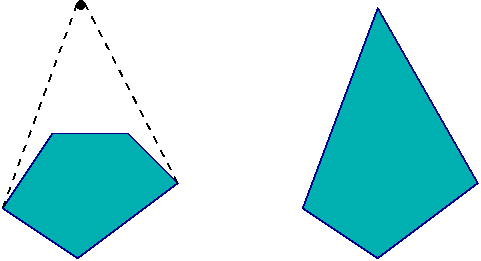
\includegraphics[scale=0.6]{images/conv_a_2}
\end{center}
\vspace*{-8mm}
\caption{Изменение выпуклой оболочки при добавлении точки}\label{fig:conv_light}
\end{figure}

Для получения новой оболочки необходимо удалить все освещённые рёбра, а концы
оставшейся ломаной соединить двумя новыми рёбрами с добавляемой точкой $x$.
Если добавляемая точка лежит на продолжении одного из рёбер, то оболочка должна
измениться, поэтому ребро, на продолжении которого лежит точка $x$, мы также будем
считать освещённым.

\newpage

Для вычисления функции $g$~---количества острых углов в выпуклой оболочке нам необходимо хранить \emph{множество} точек, углы при которых острые~(\verb|Set::@@angles| будем обозначать $A$). Случаи точки и двуугольника тривиальны (0 и 2 острых угла соответственно). Для треугольника достаточно напрямую проверить, являются ли углы острыми при помощи сравнения скалярного произведения с нулём (метод точки \verb|ac_angle?(a,b)|~--- двухместный предикат "угол образуемый точкой-вершиной и точками \verb|a|, \verb|b| острый") и если углы острые, добавить точки в множество $A$.

Для выпуклой оболочки из более чем 3 точек алгоритм вычисления количества острых углов такой: 
\begin{itemize}
\item Если точка удаляется при добавлении новой вершины в выпуклую оболочку, удалить её из множества $A$.
\item После удаления всех освещённых из добавляемой вершин следует добавить в $A$ вершины, смежные с добавленной и обладающие острым углом и добавляемую вершину, если угол при ней острый. Естественно также нужно исключить из $A$ те из смежных с добавляемой точек, углы при которых не острые. (см.~рис.~\ref{fig:conv_light})
\end{itemize}

Далее рассмотрим задачу вычисления функции $h$~--- расстояния от выпуклой оболочки до стандартного прямоугольника.\footnote{Подробный код методов реализующих эту задачу доступен в приложении А.} 

Расчёт расстояния от точки до прямоугольника и от отрезка до прямоугольника как подзадача входит в  расчёт для выпуклой оболочки, поэтому здесь рассмотрен не будет. Рассмотрение метода вычисления расстояния до отрезка рассмотрено в разделе \emph{Используемые алгоритмы и структуры данных}. 

В случае треугольника достаточно проверить расстояние от каждой стороны, если центр прямоугольника
 не лежит внутри треугольника, если центр внутри, то $g$ автоматически становится $0$, так как 
 выпуклая оболочка включает в себя свою внутренность.

Рассмотрим случай общей выпуклой оболочки:
учитывая что расстояние до выпуклой оболочки может только уменьшаться, нам нужно лишь проверить, не попадает ли прямоугольник в получаемую при добавлении вершины область, и вычислить расстояние до добавляемых отрезков.

Таким образом мы знаем как индуктивно вычислять расстояние от выпуклой оболочки до стандартного прямоугольника.

\begin{figure}[ht!]
\begin{center}
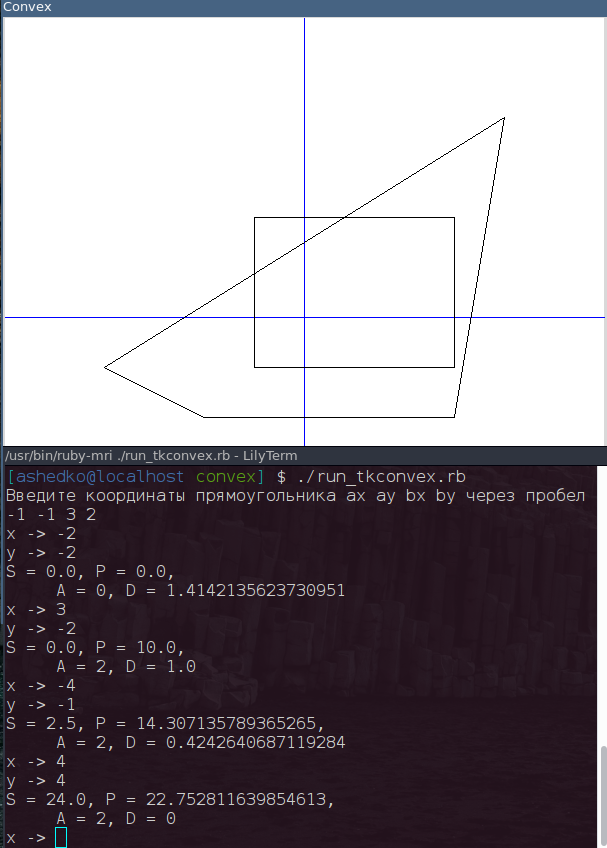
\includegraphics[scale=0.6]{images/convex_ill}
\end{center}
\vspace*{-8mm}
\caption{Иллюстрация работы программы}\label{fig:conv_ill}
\end{figure}

\newpage
\subsection{Используемые алгоритмы и структуры данных}

\textbf{Структуры данных}

Дек~(двухсвязный список), используемый в эталонном проекте не нуждается в пояснениях.

При вычислении количества острых углов используется структура данных \emph{множество}. По своей сути она представляет собой хэш, в котором ключи и есть данные. В работе она используется из-за простоты добавления и удаления элементов, так как \verb|Set| в языке Ruby позволяет выполнять над собой стандартные теоретико-множественные операции.

\textbf{Вычисление расстояния от отрезка до прямоугольника}

Прежде чем начать работу с отрезком проверим его на пересечение с прямоугольником.~(алгоритм описан ниже)
В начале вычислим положение концов отрезка относительно прямоугольника, воспользовавшись таблицей,
\begin{center}
\begin{tabular}{|c|c|}
\hline
Характеристика & Номер четверти \\
\hline 
$(\mathbf{0},\mathbf{0})$ & 0 \\ 
\hline 
$(\mathbf{0},\mathbf{1})$ & 1 \\
\hline
$(\mathbf{1},\mathbf{0})$ & 2 \\
\hline
$(\mathbf{1},\mathbf{1})$ & 3 \\
\hline
\end{tabular} 
\end{center}
где характеристика~--- результат сравнения координат точки с  координатами центра прямоугольника~(первая координата~--- горизонтальная, вторая~--- вертикальная; см.~рисунок \ref{fig:conv_rect}).
\begin{figure}[ht!]
\begin{center}
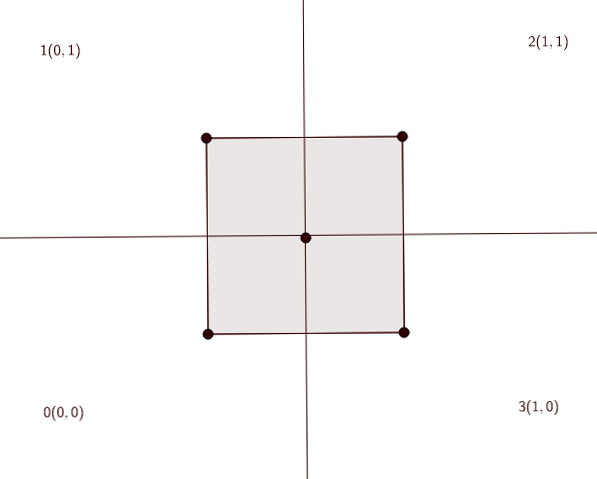
\includegraphics[scale=0.4]{images/conv_rect}
\end{center}
\vspace*{-8mm}
\caption{Разделение пространства вокруг прямоугольника}\label{fig:conv_rect}
\end{figure}

Затем проверим  не является ли отрезок точкой, и если является, остаётся только проверить расстояние до ближайших двух сторон прямоугольника при помощи метода вычисления расстояния от точки до отрезка.

Если же отрезок невырожденный, возможно 3 случая его положения относительно прямоугольника~(Рис. \ref{fig:conv_case})
\begin{list}{a}{}
\item[\textbf{a})] оба конца лежат в одной четверти;
\item[\textbf{b})] концы в соседних четвертях;
\item[\textbf{c})] концы в противоположных четвертях.
\end{list}
В случае \textbf{a} необходимо вычислить: расстояние от отрезка до ближайшей вершины прямоугольника и расстояния от концов отрезка до соответствующих им сторон прямоугольника~
(см.~приложение А) после чего взять минимальное из них
В случае \textbf{b} необходимо вычислить: расстояние от отрезка до вершин прямоугольника в соответствующих четвертях и расстояния от концов отрезка до стороны прямоугольника. Далее аналогично \textbf{a} взять минимальное расстояние.
В случае \textbf{c} нужно всего лишь взять меньшее из расстояний от вершин, не лежащих в одной четверти с концами отрезка, до отрезка.
\begin{figure}[ht!]
\begin{center}
\textbf{a})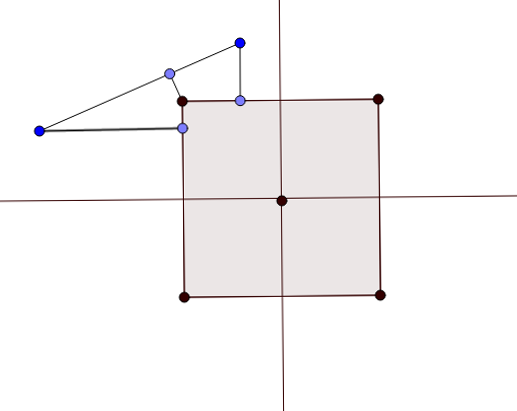
\includegraphics[scale=0.3]{images/conv_case1}
\vspace*{+10mm}
\textbf{b})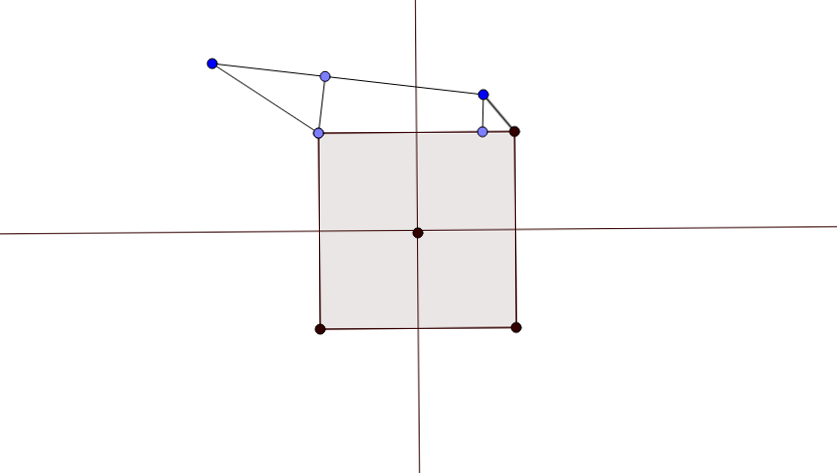
\includegraphics[scale=0.27]{images/conv_case2}
\textbf{c})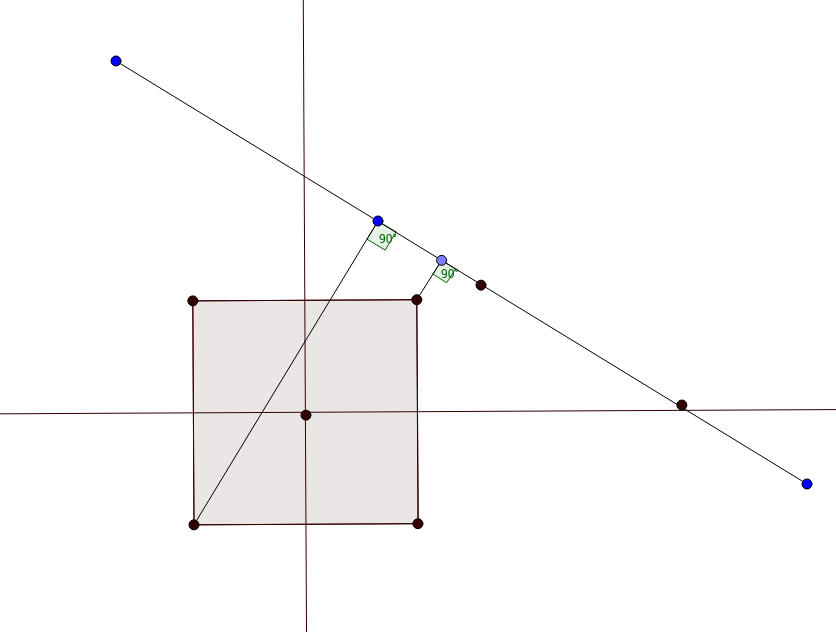
\includegraphics[scale=0.26]{images/conv_case3}
\end{center}
\vspace*{-8mm}
\caption{Различные варианты расположения точек}\label{fig:conv_case}
\end{figure}

Таким образом можно быстро находить расстояние от отрезка до прямоугольника. В данном случае задача упрощается тем, что если отрезок целиком внутри прямоугольника, то расстояние до него равно $0$. 

Выгода по сравнению с <<лобовым>> методом методом проверки алгоритм работает примерно в 3 раза быстрее (в <<лобовом>> методе производится $12$ операций вычисления длины, этот алгоритм позволяет ограничиться $4$)
Идея алгоритма автором найдена в заметках конференции, посвящённой базам данных \cite{seginters}


\textbf{Вычисление пересечения отрезка и прямоугольника~(\emph{segment clipping})}

Алгоритм Лианга-Барского~\cite{barsky} использует параметрическое уравнение прямой и неравенства, описывающие прямоугольник~(clipping window), для вычисления пересечений между прямой и прямоугольником. С помощью этих пересечений можно выяснить какая часть отрезка пересекает прямоугольник.

Параметрическое уравнение прямой:
$$x = x_0 + u (x_1 - x_0) = x_0 + t \Delta x\,\!$$
$$y = y_0 + u (y_1 - y_0) = y_0 + t \Delta y\,\!$$
Точка находится внутри прямоугольника, если:
$x_{\text{min}} \leqslant x_0 + t \Delta x \leqslant x_{\text{max}}\,\!$
и
$y_{\text{min}} \leqslant y_0 + t \Delta y \leqslant y_{\text{max}}\,\!$
, где:

\begin{tabular}{l}
$p_1 = -\Delta x  , q_1 = x_0 - x_{\text{min}}\,\!$ \\
$p_2 = \Delta x  ,  q_2 = x_{\text{max}} - x_0\,\!$\\
$p_3 = -\Delta y , q_3 = y_0 - y_\text{min}\,\!$\\
$p_4 = \Delta y ,  q_4 = y_\text{max} - y_0\,\! $
\end{tabular}

Чтобы получить пересечение, нужно учесть следующее.
\begin{enumerate}
\item Если отрезок параллелен $i$-тому ребру $p_i=0$  для этого ребра.
\item Если для этого $i,q_i<0$, отрезок полностью находится вне прямоугольника.
\item Когда $p_i<0$ отрезок направлен внутрь через это ребро, а если $p_i>0$~---наружу.
\item Для ненулевого $p_k$, $u=\frac{q_i}{p_i}$ даёт точку пересечения.
\item Вычислить $u_1$, $u_2$. Для $u_1$, посмотреть на рёбра, где  $p_i<0$. $u_1$~--- максимум из $\left\{0,{q_i}/{p_i}\right\}$.Для $u_2$, посмотреть на $p_i>0$. $u_2$~---минимум из $\left\{1,{q_i}/{p_i}\right\}$. Если $u_1>u_2$, то отрезок находится снаружи и потому также не пересекает прямоугольник.
\end{enumerate}

\subsection{Возможные обобщения}
В качестве более общей задачи можно рассматривать:
\begin{itemize}
\item задачу в пространстве произвольной размерности;
\item прямоугольник общего положения~(решается при помощи преобразования поворота и сдвига для координат точек);
\item поиск расстояния до других фигур~(круг, треугольник, произвольная область ограниченная конечным числом ломанных). Возможное решение~--- конформное отображение.
\end{itemize}


\section{Модификация проекта «Изображение проекции полиэдра»}

\subsection{Постановка задачи}

Все рёбра делятся на три класса: \emph{полностью видимые}, \emph{видимые частично} и \emph{полностью невидимые}. Назовём грань «гранью с полностью видимыми рёбрами», если все образующие её рёбра полностью видимы. Если все образующие грань рёбра полностью невидимы, то грань будем называть «гранью с полностью невидимыми рёбрами». Все остальные грани будем называть «гранями с частично видимыми рёбрами». Модифицируйте эталонный проект таким образом, чтобы определялась и печаталась следующая характеристика полиэдра: \emph{сумма периметров проекций «граней с частично видимыми рёбрами», проекция центра которых находится строго вне квадрата единичной площади с центром в начале координат и сторонами, параллельными координатным осям}.
~(28).

\subsection{Теоретические аспекты}

Задача изображения проекции полиэдра без невидимых рёбер может быть решена следующим образом: будем отображать отрезки~--- проекции рёбер полиэдра, причём части рёбер, \emph{затенённые} гранями полиэдра, учитывать не нужно.
Полиэдр задаётся тремя наборами: вершин, рёбер, граней, соответствием между ними и вращением трёхмерного пространства. Проектирование производится при помощи бесконечной перспективы~(Физическая интерпретация: свет падает на объект из бесконечно удалённой точки параллельным потоком и мы видим тень объекта на плоскости, перпендикулярной вектору направления света). Далее вектор направления света будем называть \emph{вектором проектирования}.

Механизм проектирования предельно прост: после преобразования координат~(пространственный поворот на соответствующие углы Эйлера и гомотетия) для отображения точки достаточно лишь \emph{забыть} её $z$-координату.

Вкратце опишем алгоритм \emph{затенения} ребра гранью:
Рассмотрим произвольное ребро. Каждая грань разбивает его на \emph{затенённые} и \emph{освещённые} участки. Несложно показать что в нашем случае~(грани-выпуклые многоугольники) освещённая часть представляет собой либо ребро, либо $\O$.~(см. рис.\ref{fig:poly_shadow})

\begin{figure}[ht!]
\begin{center}
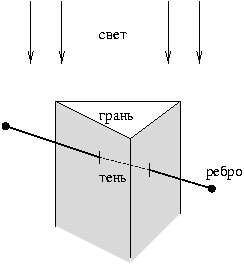
\includegraphics[scale=1]{images/pol_shad.png}
\caption{Затенение ребра гранью} \label{fig:poly_shadow}
\end{center}
\end{figure}

Для получения конечного результата необходимо учесть тени от всех граней~(Утверждение открывает широкий простор для оптимизации~--- нахождения достаточного условия). 

Воспользовавшись тем фактом что ребро~--- одномерный объект, задачу нахождения пересечения освещённых областей от всех граней можно свести к задаче поиска дополнения покрытия интервала $(0,1)$ набором других интервалов. Тень от грани~--- пересечение ребра и открытой бесконечной призмы, сверху ограниченной гранью, а с <<боков>>~--- плоскостями, содержащими рёбра грани и вектор проектирования, нормали которых направлены внутрь призмы. Процесс построения призмы показан на рисунке \ref{fig:poly_prism}.

\begin{figure}[ht!]
\begin{center}
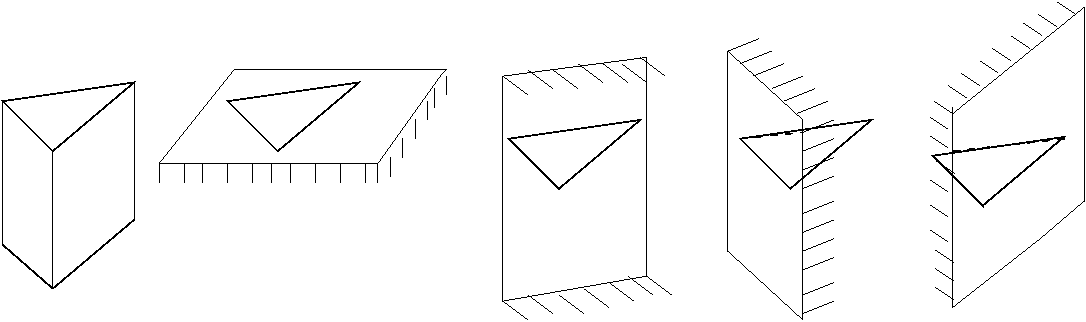
\includegraphics[scale=0.6]{images/pol_prism.png}
\caption{Построение призмы затенения} \label{fig:poly_prism}
\end{center}
\end{figure}

\subsection{Детали реализации}

Таким образом мы можем сказать какие рёбра будут \emph{видимыми}, а какие \emph{невидимыми}, что соответственно позволяет нам определить какие гани являются \emph{частично видимыми}.

Метод грани, решающий эту задачу:
\begin{lstlisting}
class Facet
    
    ...

  def part_vis?
    return false if !@edges
    pr1,pr2 = true, true
    trtab = @edges.map{|edge| [edge.compl_visible?,edge.invisible?]}
    trtab.each{|x|pr1&&=x[0];pr2&&=x[1]}
    !(pr1||pr2)
  end 
end
\end{lstlisting}

Естественно для этого требуется знать какие рёбра принадлежат грани. Воспользуемся структурой данных <<хэш>> для удаления дубликатов рёбер и затем поставим каждой грани в соответствие набор рёбер, ей принадлежащих. Это можно сделать при помощи простой проверки что множество вершин грани содержит концы ребра.
\begin{lstlisting}
  def edges_uniq
    edges = {}
    @edges.each do |e|
      if edges[[e.beg, e.fin]].nil? && edges[[e.fin, e.beg]].nil?
        edges[[e.beg, e.fin]] = e
      end
    end
    @edges = edges.values
  end
\end{lstlisting}

Наконец, для определения положения центра грани необходимо проверить что его координаты  в изначальной системе отсчёта соответствуют неравенствам:
$|x_c|>0,5$ и $|y_c|>0,5$. Откуда следует что параметры проектирования должны быть известны в классе \verb|Polyedr|. 
Код метода, решающего эту задачу:
\begin{lstlisting}
  def outside_sqr?(alpha,beta,gamma,c)
    cent = center
    cent = cent.rz(-gamma).ry(-beta).rz(-alpha)*(1/c)
    (cent.x>0.5||cent.x<-0.5)&&(cent.y>0.5||cent.y<-0.5)
  end
\end{lstlisting}

В итоге все методы, требующиеся для решения поставленной задачи описаны и остаётся только проверить все грани на соответствие условиям задачи и сложить периметры граней им удовлетворяющих.
На рисунке \ref{fig:poly_fig} представлен результат работы программы, где точками отмечены центры граней, удовлетворяющих условиям задачи.

\subsection{Возможные обобщения}
Задачу можно обобщить, например, потребовав покрывать грани какой-либо текстурой и описывать условия задачи с учётом текстуры. Другой задачей может быть поиск суммы расстояний между правильными пирамидами. построенными на гранях полиэдра, как на основаниях.

\begin{figure}[ht!]
\begin{center}
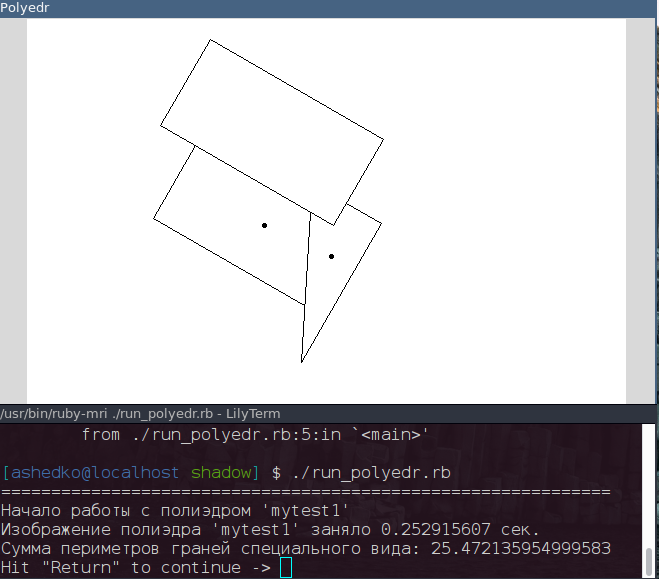
\includegraphics[scale=0.8]{images/poly_1.png}
\caption{Иллюстрация работы программы} \label{fig:poly_fig}
\end{center}
\end{figure}
\begin{thebibliography}{}

\bibitem{convex}
\link{https://home.mephi.ru/files/2373/material\_ici\_toc.zip/index.html}~---
Описание проекта «Выпуклая оболочка».

\bibitem{seginters}
{\em Advances in Spatial and Temporal Databases: 9th International Symposium.}~---
SSTD 2005, Angra Dos Reis Brazil, August 22-24, 2005, Proceedings, Стр.~333.

\bibitem{barsky}
Liang, Y.D., and Barsky, B., {\em A New Concept and Method for Line Clipping.}~---
ACM Transactions on Graphics, 3(1):1-22, January 1984.

\bibitem{ruby}
\link{http://ru.wikipedia.org/wiki/Ruby}~---
Википедия (свободная энциклопедия) о языке Ruby.

\bibitem{polyedr}
\link{https://home.mephi.ru/files/3214/material\_ici\_toc.zip/index.html}~---
Описание проекта «Изображение проекции полиэдра».

\bibitem{rlatex}
С.М. Львовский.
{\em Набор и вёрстка в системе \LaTeX, 3-е изд., испр. и доп.}~---
М., МЦНМО, 2003. Доступны исходные тексты этой книги.

\bibitem{texbook}
D.~E.~Knuth. {\em The \TeX book.}~---
Addison-Wesley, 1984. Русский перевод:
Дональд~Е.~Кнут.
{\em Все про \TeX.}~--- Протвино, РД\TeX, 1993.

\bibitem{compf}
\link{https://home.mephi.ru/files/2077/material\_ici\_toc.zip/index.html}~---
Описание проекта \emph{<<Стековый компилятор формул>>}
Е.А. Роганов


\bibitem{rubydoc}
\link{http://ruby-doc.org/}~---
Документация языка Ruby


\end{thebibliography}

%\newpage
%\section{Приложение А}

Проект <<Выпуклая оболочка>>. Методы, отвечающие за вычисление расстояния от отрезка до прямоугольника.

\lstinputlisting[numbers=none, linerange={1-125}]{programms/r2point.rb}

%\section{Приложение Б}

\begin{enumerate}

\item
Так как используемый по умолчанию для просмотра pdf-файлов Adobe Reader не 
поддерживает возможности перезагрузки модифицированной версии документа, то
необходимо создать в своей домашней директории файл \verb|.latexmkrc|
со следующей строкой (без начальных пробелов):

\begin{verbatim}
  $pdf_previewer= "start evince";
\end{verbatim} 

\item
Для получения и просмотра итогового документа необходимо выполнить команду

\begin{verbatim}
 latexmk -pdf -pvc paper.tex
\end{verbatim} 

\noindent
Скрипт \verb|latexmk| анализирует время модификации всех файлов, от которых
зависит итоговый документ \verb|paper.pdf|; выполняет при необходимости
нужное количество раз команду \verb|pdflatex paper.tex|; запускает программу,
позволяющую увидеть итоговый документ, или посылает этой программе
сигнал о необходимости перезагрузки модифицированной версии документа. 

\item
Обязательно следует соблюдать рекомендации по набору русского языка, 
оформлению рисунков, таблиц, текстов алгоритмов и программ, сформулированные
в шаблоне пояснительной записки.

\item
Объём пояснительной записки к курсовой работе должен быть не менее
20 страниц (включая титульный лист, аннотацию, содержание, введение,
основные разделы, список литературы и интернет-ресурсов, приложения).

\item
Пояснительная записка не должна содержать сколь-либо объёмных фрагментов
текста, заимствованных из каких-либо источников. 

\item
Настоятельно рекомендуется следить за сообщениями об ошибках и 
предупреждениях, появляющихся в файле \verb|paper.log|, и исправлять их.

\item
Если Вы захотите установить/использовать \TeX на своём домашнем компьютере,
то ознакомьтесь с рекомендациями, размещёнными в сети Интернет по адресу
\link{http://www.tug.org/texlive/doc/texlive-ru/texlive-ru.html}.

\end{enumerate}


\end{document}
